\documentclass[10pt]{beamer}
\usefonttheme{professionalfonts,serif}
\def\newblock{\hskip .11em plus .33em minus .07em}
\usepackage[numbers,sort]{natbib}
\renewcommand{\rmdefault}{psbx}
\usepackage[utf8]{inputenc}
\usepackage[T1]{fontenc}
\usepackage{textcomp}
\usepackage{eulervm}

\usetheme{default}           % tips from David Blei
\useinnertheme{circles}
\useoutertheme{infolines}
\setbeamertemplate{headline}{}
\setbeamertemplate{navigation symbols}{}
\setbeamerfont{itemize/enumerate subbody}{size=\normalsize}
\setbeamerfont{itemize/enumerate subsubbody}{size=\normalsize}
\usecolortheme{seahorse}
\setbeamersize{text margin left=2mm,text margin right=2mm}

\graphicspath{{../../figures/}}

\definecolor{mypine}{rgb}{0.05,0.45,0.05}
\definecolor{mycyan}{rgb}{0.0,0.9,0.9}
\newcommand{\Red}{\textcolor{red}}
\newcommand{\Blue}{\textcolor{blue}}
\newcommand{\Green}{\textcolor{mypine}}
\newcommand{\PineGreen}{\textcolor{mypine}}
\newcommand{\Magenta}{\textcolor{magenta}}
\newcommand{\Cyan}{\textcolor{mycyan}}

\newcommand{\N}{\mathcal{N}}
\newcommand{\R}{\mathbb{R}}
\newcommand{\T}{{\scriptsize^{\top}}}
\newcommand{\D}{\mathcal{D}}
\newcommand{\F}{\mathcal{F}}
\newcommand{\E}{\mathbb{E}}
\newcommand{\V}{\mathbb{V}}
\newcommand{\M}{\mathcal{M}}
\newcommand{\KL}{\mathcal{KL}}
\newcommand{\cut}[1]{}
\newcommand{\trace}{\operatorname{trace}}

\newcommand{\bmu}{{\boldsymbol{\mu}}}
\newcommand{\btheta}{\boldsymbol{\theta}}
\newcommand{\bepsilon}{\boldsymbol{\epsilon}}
\newcommand{\balpha}{\boldsymbol{\alpha}}
\newcommand{\bbeta}{\boldsymbol{\beta}}
\newcommand{\bphi}{\boldsymbol{\phi}}
\newcommand{\bPhi}{\boldsymbol{\Phi}}
\newcommand{\bSigma}{\boldsymbol{\Sigma}}
\newcommand{\bpi}{\boldsymbol{\pi}}
\newcommand{\blambda}{\boldsymbol{\lambda}}

\newcommand{\argmax}{\operatorname{argmax}}
\newcommand{\argmin}{\operatorname{argmin}}
\newcommand{\ci}{{\bot\negthickspace\negthickspace\bot}} % conditional indep.
\newcommand{\neigh}{\operatorname{ne}}
\newcommand{\vectr}[2]{  \left[ \!\!\begin{array}{c} #1 \\
      #2 \end{array} \!\!\right]}
\newcommand{\deff}{\stackrel{\mathrm{def}}{=}}
\newcommand{\deldel}[2]{\frac{\partial #1}{\partial #2}}

\newcommand{\maketilde}{\raisebox{0.4ex}{\tiny $\sim$}}
\newcommand{\bfa}{\mathbf a}
\newcommand{\bfb}{\mathbf b}
\newcommand{\bfe}{\mathbf e}
\newcommand{\bff}{\mathbf f}
\newcommand{\bfk}{\mathbf k}
\newcommand{\bfm}{\mathbf m}
\newcommand{\bfn}{\mathbf n}
\newcommand{\bfp}{\mathbf{p}}
\newcommand{\bfs}{\mathbf s}
\newcommand{\bfu}{\mathbf u}
\newcommand{\bfx}{\mathbf x}
\newcommand{\bfy}{\mathbf y}
\newcommand{\bft}{\mathbf t}
\newcommand{\bfv}{\mathbf v}
\newcommand{\bfw}{\mathbf w}
\newcommand{\bfA}{\mathbf A}
\newcommand{\bfI}{\mathbf I}
\newcommand{\bfK}{\mathbf K}


\title{Discrete Categorical Distribution}
\author{Carl Edward Rasmussen}
\date{November 11th, 2016}

\begin{document}


\begin{frame}
\titlepage
\end{frame}


\begin{frame}
\frametitle{Key concepts}

We generalize the concepts from binary variables to multiple discrete
outcomes.

\begin{itemize}
\item discrete and multinomial distributions
\item the Dirichlet distribution
\end{itemize}
\end{frame}


\begin{frame}
\frametitle{The multinomial distribution (1)}

\centerline{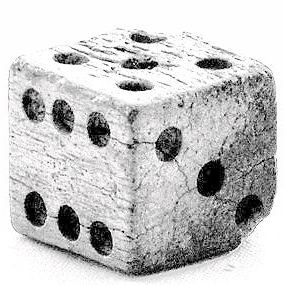
\includegraphics[width=0.19\textwidth]{die}}

Generalisation of the binomial distribution from 2 outcomes to $m$ outcomes.\\
Useful for random variables that take one of a finite set of possible outcomes. 

Throw a die $n=60$ times, and count the observed (6 possible) outcomes.
\begin{center}
\parbox{0.35\textwidth}{
\begin{tabular}{l l}
Outcome & Count\\
\hline
$X=x_1=1$ & $k_1=12$\\
$X=x_2=2$ & $k_2=7$\\
$X=x_3=3$ & $k_3=11$\\
$X=x_4=4$ & $k_4=8$\\
$X=x_5=5$ & $k_5=9$\\
$X=x_6=6$ & $k_6=13$\\
\hline
\end{tabular}
}
\parbox{0.58\textwidth}{
Note that we have one parameter too many. We don't need to know all
the $k_i$  and $n$, because $\sum_{i=1}^6 k_i=n$. 
}
\end{center}

\end{frame}

\begin{frame}
\frametitle{The multinomial distribution (2)}

Consider a discrete random variable $X$ that can take one of $m$
values $x_1,\ldots,x_m$.

Out of $n$ independent trials, let $k_i$ be the number of
times $X=x_i$ was observed.\\
It follows that $\sum_{i=1}^m k_i=n$.

Denote by $\pi_i$ the probability that $X=x_i$, with
$\sum_{i=1}^m \pi_i=1$.

The probability of observing a vector of occurrences
$\bfk=[k_1,\ldots,k_m]^\top$ is given by the \Blue{\emph{multinomial
distribution}} parametrised by $\bpi=[\pi_1,\ldots,\pi_m]^\top$:
%
\[
p(\bfk|\bpi,n)\;=\; p(k_1,\ldots,k_m|\pi_1,\ldots,\pi_m,n) 
\;=\;\frac{n!}{k_1!k_2!\ldots k_m!}\prod_{i=1} \pi_i^{k_i}
\]
\vspace*{-2ex}
\begin{itemize}
\item Note that we can write $p(\bfk|\bpi)$ since $n$ is redundant.
\item The multinomial coefficient $\frac{n!}{k_1!k_2!\ldots k_m!}$ is a
 generalisation of
 $\big(\!\!\begin{array}{c}n\\k\end{array}\!\!\big)$.
\end{itemize}

The discrete or \Blue{\emph{categorical distribution}} is the
  generalisation of the Bernoulli to $m$ outcomes, and the special
  case of the multinomial with one trial:
\[
p(X=x_i|\bpi)\;=\;\pi_i.
\]

\end{frame}

\begin{frame}
\frametitle{Example: word counts in text}

Consider describing a text document by the frequency of occurrence of every distinct word.

The UCI \Blue{\emph{Bag of Words}} dataset from the University of California, Irvine. 
\texttt{\footnote{http://archive.ics.uci.edu/ml/machine-learning-databases/bag-of-words/}}

\end{frame}


\begin{frame}
\frametitle{Priors on multinomials: The Dirichlet distribution}

The Dirichlet distribution is to the categorical/multinomial what the Beta is to the Bernoulli/binomial.\\ 
It is a generalisation of the Beta defined on the $m-1$ dimensional simplex.

\parbox{0.69\textwidth}{
\begin{itemize}
\item Consider the vector $\bpi=[\pi_1,\ldots,\pi_m]^\top$, with $\sum_{i=1}^m \pi_i=1$ 
and $\pi_i\in(0,1)\;\; \forall i$.
\item Vector $\bpi$ lives in the open standard $m-1$ simplex.
\item $\bpi$ could for example be the parameter vector of a multinomial.
\hfill[Figure on the right $m=3$.]
\end{itemize}
}
\parbox{0.3\textwidth}{
\centerline{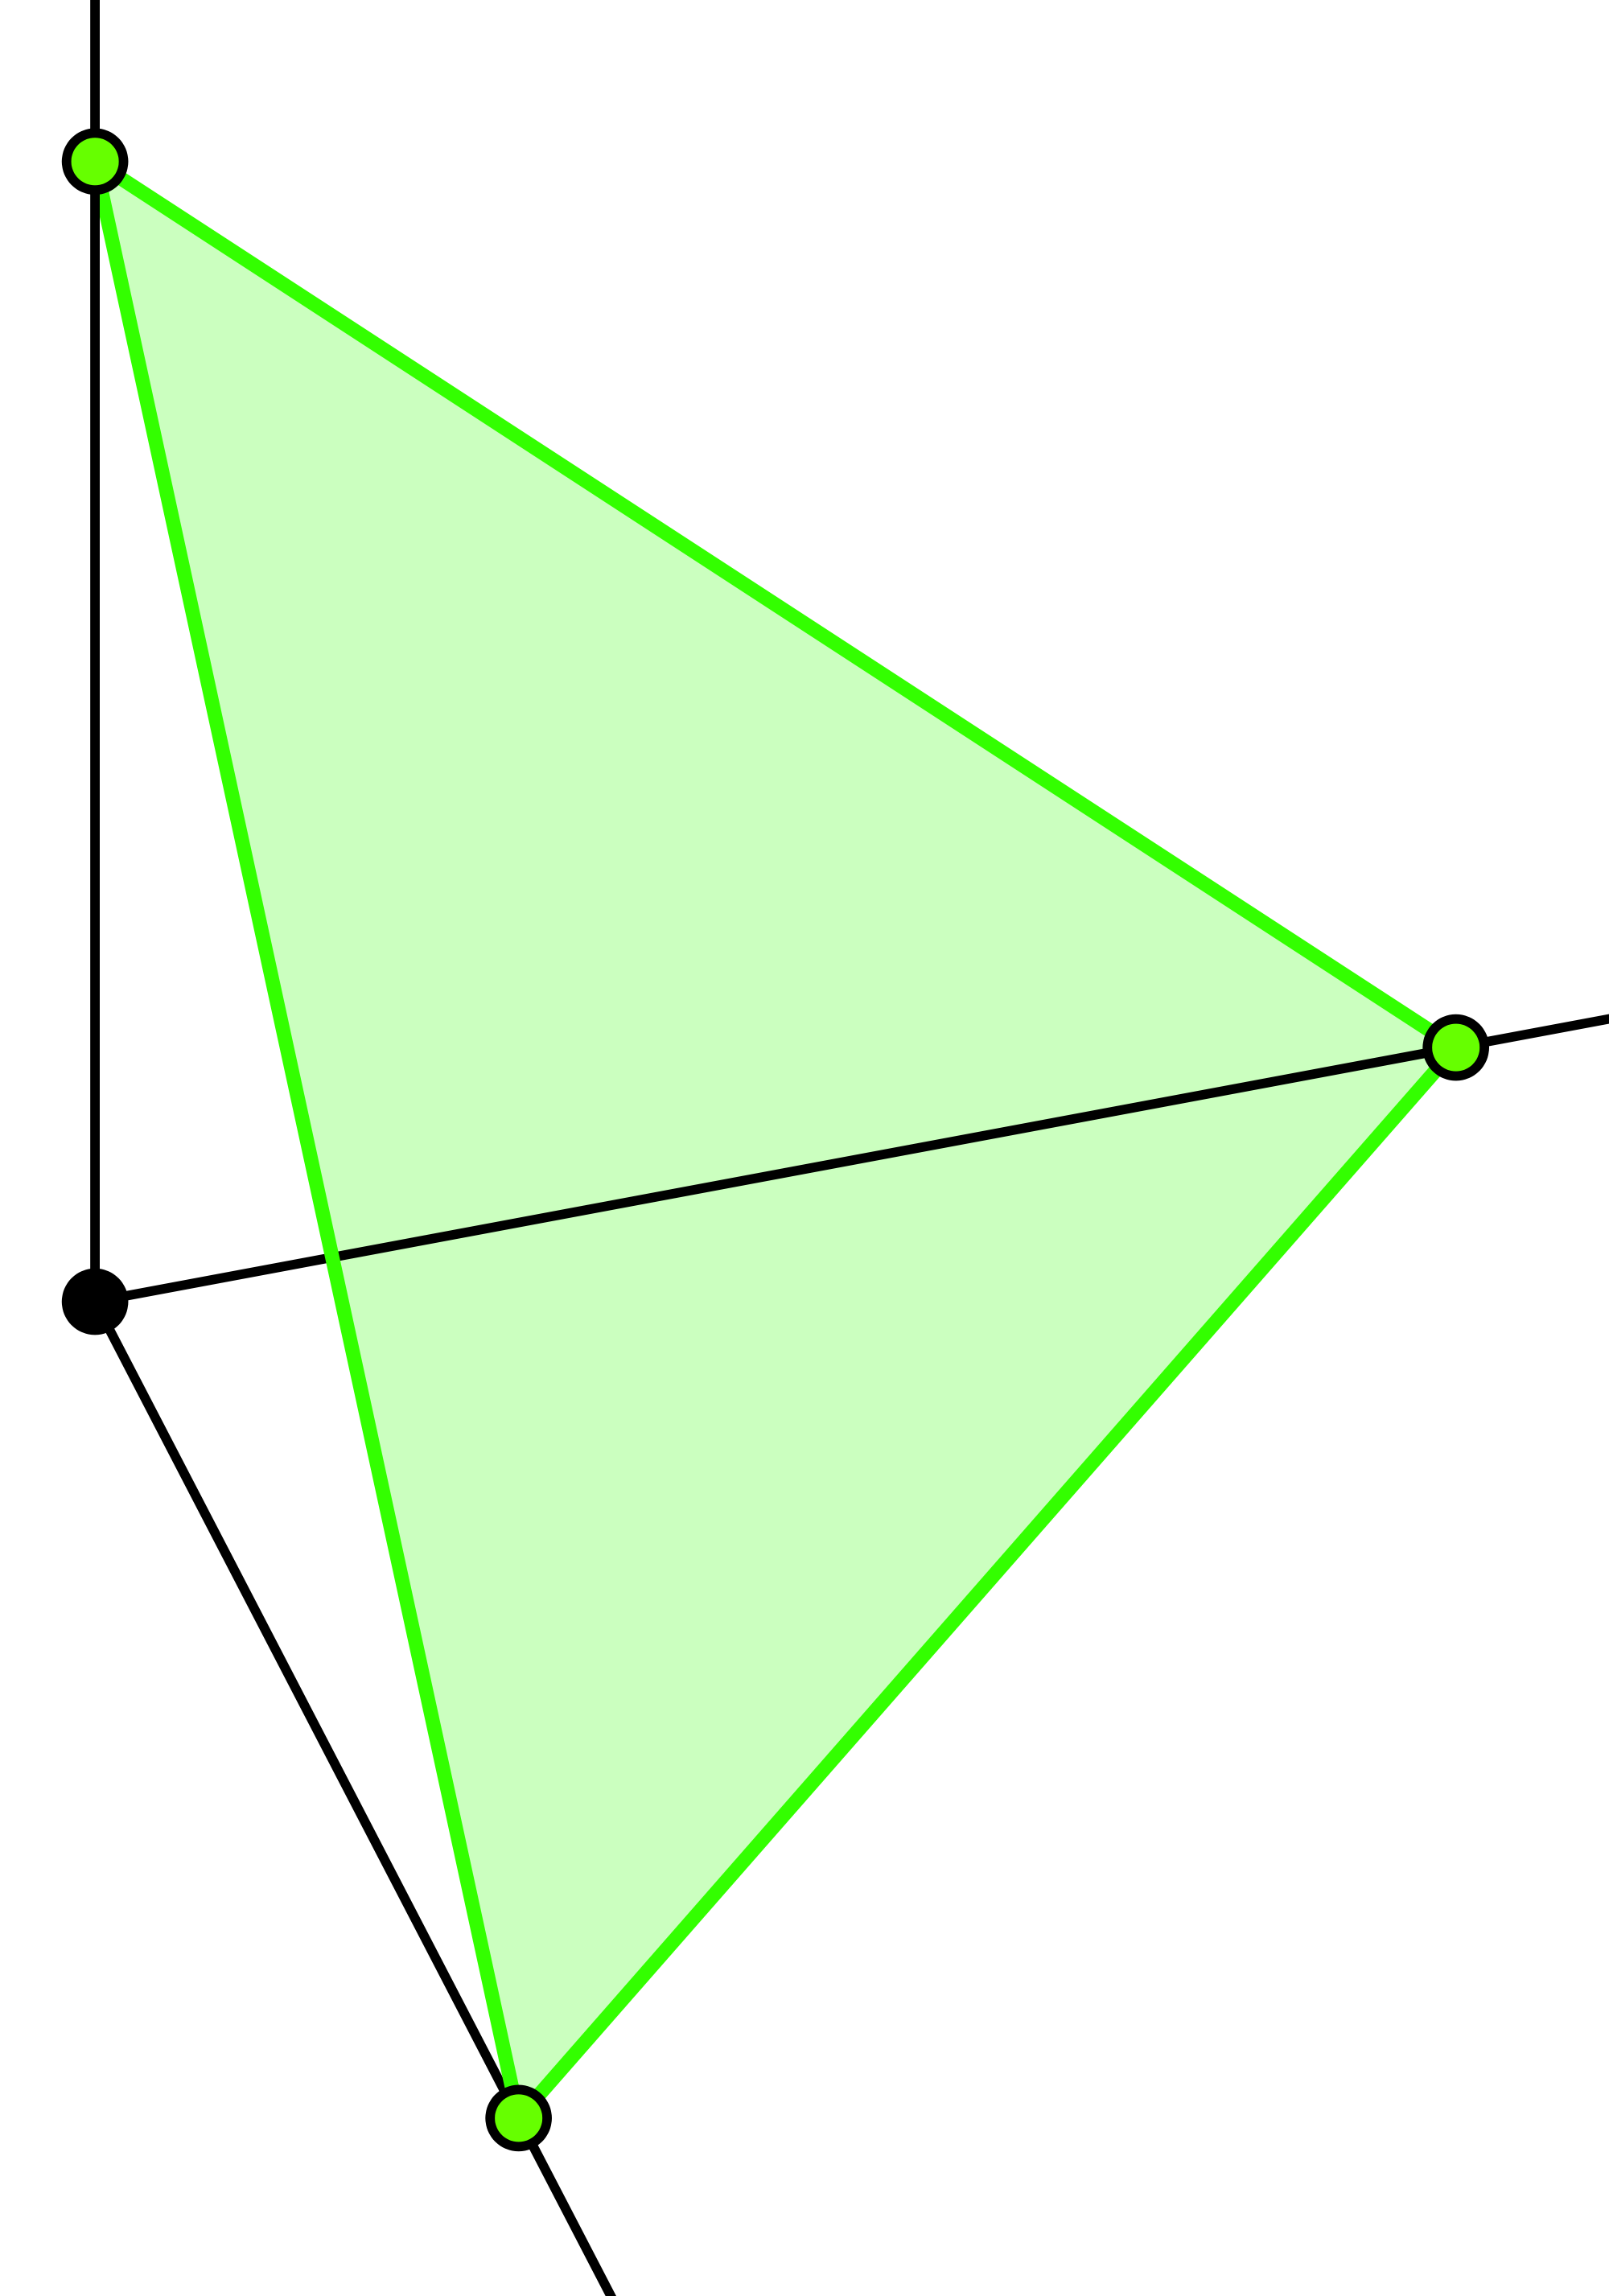
\includegraphics[width=0.15\textwidth]{2D-simplex}}
}

The Dirichlet distribution is given by
\[
\mathrm{Dir}(\bpi|\alpha_1,\ldots,\alpha_m)\;=\;
\frac{\Gamma(\sum_{i=1}^m\alpha_i)}{\prod_{i=1}^m\Gamma(\alpha_i)}
\prod_{i=1}^m\pi_i^{\alpha_i-1}
\;=\;\frac{1}{B(\balpha)}\prod_{i=1}^m\pi_i^{\alpha_i-1}
\]
\begin{itemize}
\item $\balpha=[\alpha_1,\ldots,\alpha_m]^\top$ are the shape parameters.
\item $B(\balpha)$ is the multivariate beta function.
\item $E(\pi_j)=\tfrac{\alpha_j}{\sum_{i=1}^m\alpha_i}$ is the mean for the $j$-th element.
\end{itemize}


\end{frame}


\begin{frame}
\frametitle{Dirichlet Distributions from Wikipedia}
\centerline{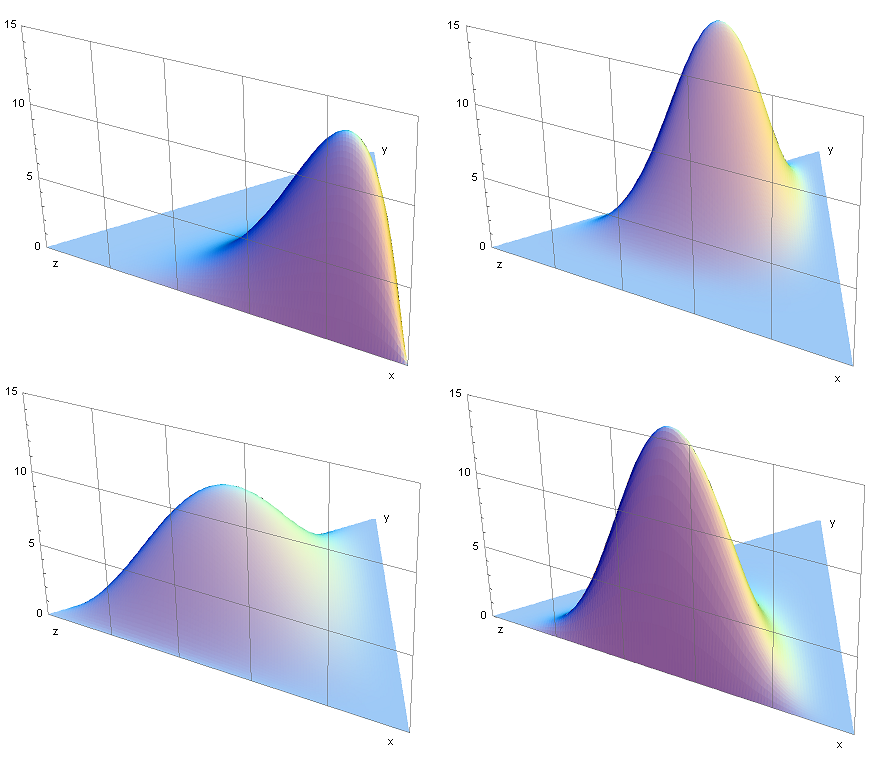
\includegraphics[width=0.75\textwidth]{Dirichlet_distributions}}
\end{frame}


\begin{frame}
\frametitle{The symmetric Dirichlet distribution}

In the symmetric Dirichlet distribution all parameters are identical:
$\alpha_i=\alpha,\;\; \forall i$.

{\small
\texttt{en.wikipedia.org/wiki/File:LogDirichletDensity-alpha\_0.3\_to\_alpha\_2.0.gif}
}

To sample from a symmetric Dirichlet in $D$ dimensions with
concentration $\alpha$ use: \texttt{w = randg(alpha,D,1); bar(w/sum(w));}\\[4mm]

\centerline{
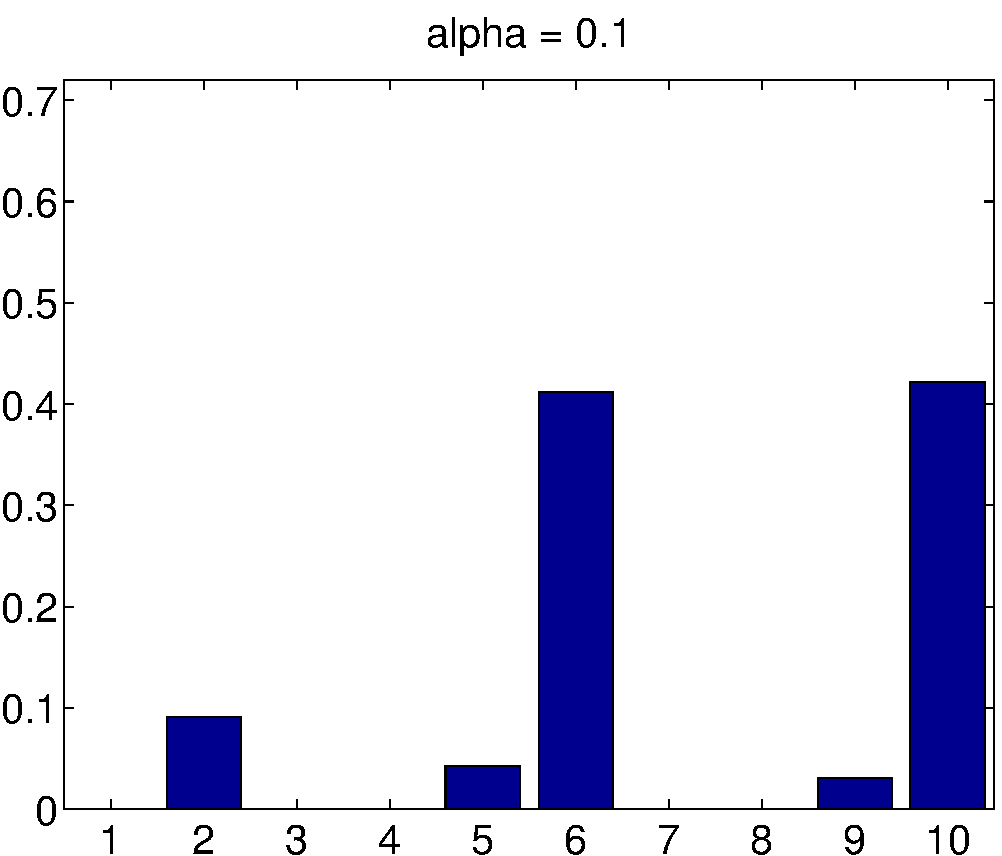
\includegraphics[width=0.3\textwidth]{dira}
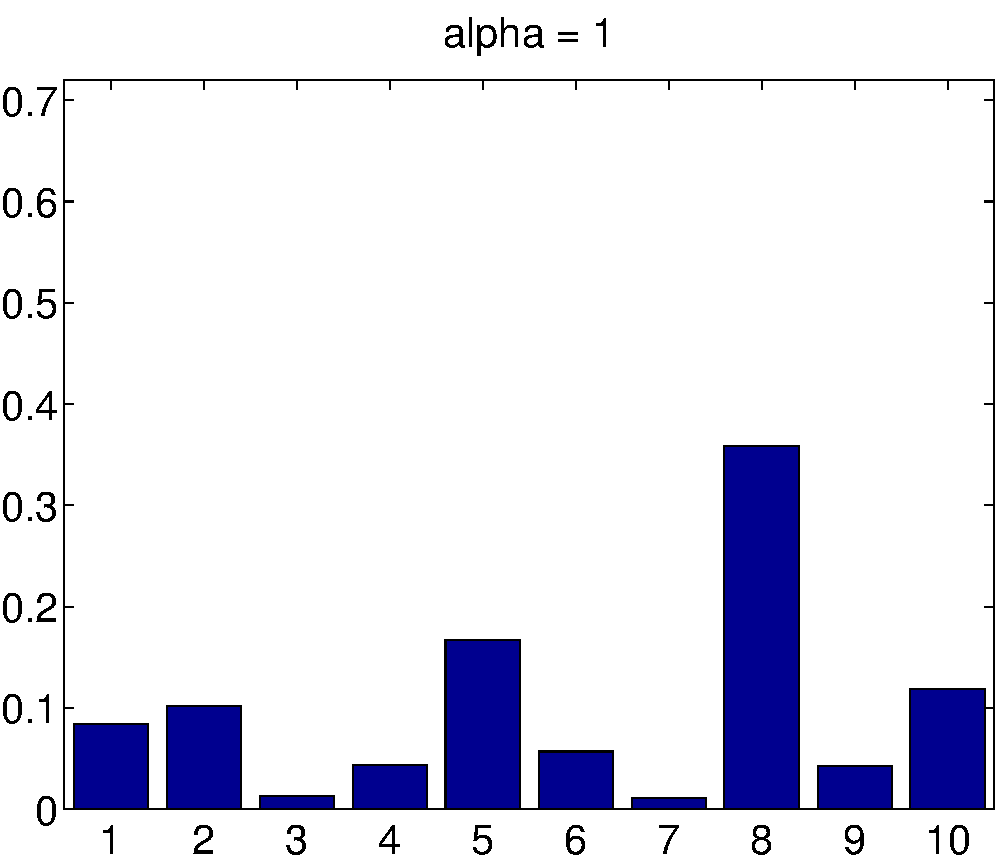
\includegraphics[width=0.3\textwidth]{dirb}
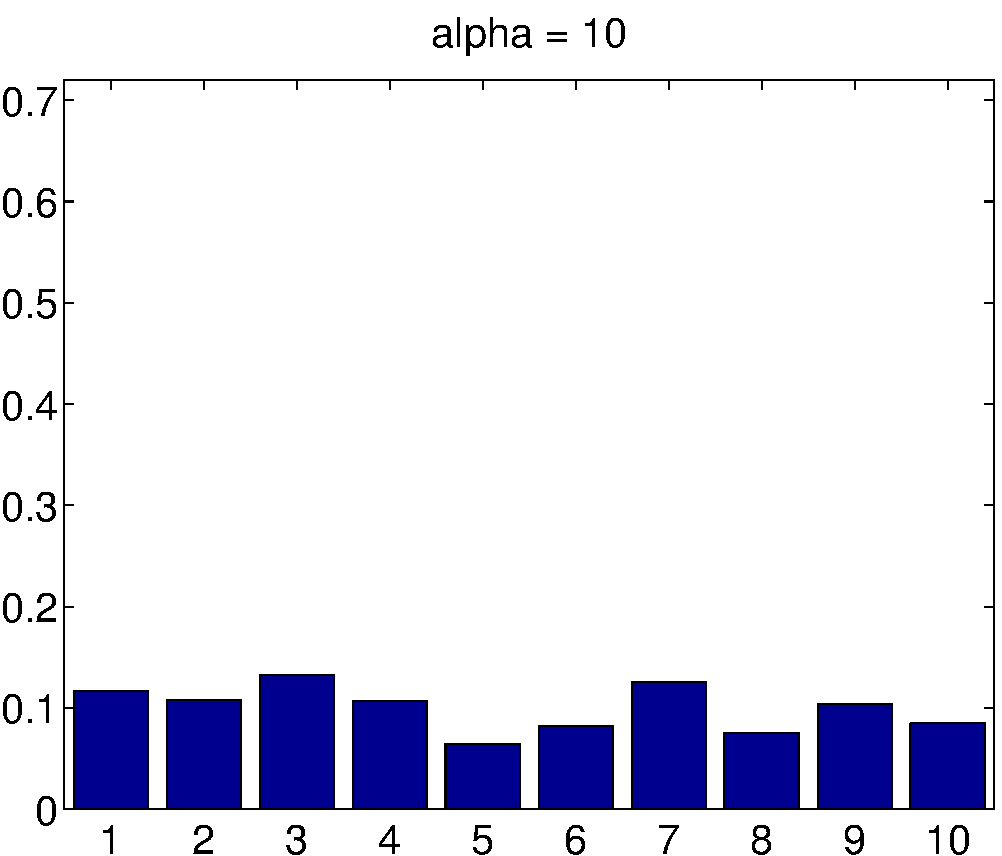
\includegraphics[width=0.3\textwidth]{dirc}
}

Distributions drawn at random from symmetric 10 dimensional Dirichlet distributions
with various concentration parameters.
\end{frame}


\end{document}